%  SigUI: User Manual
%
%  Copyright (C) 2010 Sourcefire, Inc.
%  Author: Török Edvin <edwin@clamav.net>
%
%  This program is free software; you can redistribute it and/or modify
%  it under the terms of the GNU General Public License version 2 as
%  published by the Free Software Foundation.
%
%  This program is distributed in the hope that it will be useful,
%  but WITHOUT ANY WARRANTY; without even the implied warranty of
%  MERCHANTABILITY or FITNESS FOR A PARTICULAR PURPOSE.  See the
%  GNU General Public License for more details.
%
%  You should have received a copy of the GNU General Public License
%  along with this program. If not, see <http://www.gnu.org/licenses/>.

\documentclass[a4paper,titlepage,english]{report}
\usepackage{lmodern}
\usepackage[T1]{fontenc}
\usepackage{textcomp}
\usepackage{fancyhdr}
\usepackage{longtable}
\usepackage{afterpage}
\usepackage{ifthen}
\usepackage{ifpdf}
\usepackage{titlesec}
\usepackage{microtype}
\usepackage[footnotesize,bf,justification=centering]{caption}
\usepackage[usenames, dvipsnames]{color}
%%% general setup
\usepackage[english]{babel}
\usepackage[utf8x]{inputenc}
\usepackage[perpage]{footmisc}
\usepackage{nomencl}
\usepackage{boxedminipage}
\usepackage{float}
\usepackage{algorithmic}
\usepackage{subfig}
\usepackage{moreverb}
\usepackage{prettyref}
\usepackage{url}
\usepackage{makeidx}
\usepackage{xcolor}
\usepackage{cmap}
%\makeindex
\newrefformat{cha}{Chapter~\ref{#1}}
\newrefformat{sec}{Section~\ref{#1}}
\newrefformat{sub}{Section~\ref{#1}}
\newrefformat{tab}{Table~\ref{#1}}
\newrefformat{fig}{Figure~\ref{#1}}
\newrefformat{apdx}{Appendix~\ref{#1}}

\definecolor{LinkColor1}{rgb}{0.208,0.374,0.486}
\definecolor{LinkColor2}{rgb}{0.216,0.439,0.388}

\ifpdf
% pdfLaTeX setup
    \usepackage[pdftex]{graphicx}
    \DeclareGraphicsExtensions{.pdf, .eps}   %%% standard extension for included graphics
%    \pdfminorversion=5
%    \pdfcompresslevel=9
%    \pdfobjcompresslevel=1
    \usepackage[                %%% hyper-references for pdflatex
    bookmarks=true,%                   %%% generate bookmarks ...
    bookmarksnumbered=true,%           %%% ... with numbers
    bookmarksopen = true,
    colorlinks=true,
    hyperfigures,
    linkcolor=LinkColor1,
    filecolor=LinkColor2,
    menucolor=LinkColor2,
    urlcolor=LinkColor2,
    citecolor=LinkColor1,
%    linktocpage,
    pagebackref,
    pdfpagelabels,
    pdfpagelayout=OneColumn,
    plainpages=false,
    hypertexnames=true,%              %%% needed for correct links to figures !!!
    linkbordercolor={0 0 1},           %%% blue frames around links
    pdfborder={0 0 0}]{hyperref}%      %%% pdfborder={0 0 1} is the default
    \hypersetup{
	pdfauthor = {T\"{o}r\"{o}k Edvin <edwin@clamav.net>},
	pdftitle =  {ClamAV for Windows - SigUI},
	pdfsubject = {User Manual},
	pdfkeywords = {}
    }
    \pdfadjustspacing=1                %%% force LaTeX-like character spacing
\else
    \usepackage{graphicx}
    \DeclareGraphicsExtensions{.eps,.ps}
    \usepackage{epsfig}
    \usepackage[ dvips,
                 bookmarks,
                 bookmarksopen = true,
                 bookmarksnumbered = true,
                 breaklinks = true,
                 linktocpage,
                 pagebackref,
                 colorlinks = false,
%                 hyperindex = true,
                 hyperfigures
                 ]{hyperref}

\fi

%A4 settings
\ifpdf
   \pdfpageheight=297mm
   \pdfpagewidth=210mm
\else
   \setlength{\paperheight}{297mm}
   \setlength{\paperwidth}{210mm}
\fi
\makeglossary

\floatstyle{ruled}
\newfloat{program}{thp}{lop}
\floatname{program}{Program}

%\definecolor{grey1}{gray}{0.8}
%\definecolor{grey2}{gray}{0.3}
%\definecolor{grey3}{gray}{0.6}

\definecolor{grey1}{gray}{0.8}
\definecolor{grey2}{gray}{0.3}
\definecolor{grey3}{gray}{0.6}
\definecolor{TitleColor}{rgb}{0.208,0.374,0.486}
\definecolor{NameColor}{rgb}{0.126,0.263,0.361}

% Based on Antonina Liedtke's article in Linux+ 6/2003
\def\greyp{%
    \unitlength=1mm%
    \begin{picture}(0,0)
	\put(0,-1.5){\textcolor{grey1}{\rule{13cm}{5.3mm}}\textcolor{grey2}%
	{\rule{9mm}{5.3mm}}\hss}
    \end{picture}
}
\def\greypl{%
    \unitlength=1mm%
    \begin{picture}(0,0)
	\put(0,-1.5){\textcolor{grey2}{\rule{9mm}{5.3mm}}\textcolor{grey1}%
	{\rule{13cm}{5.3mm}}\hss}
    \end{picture}
}
\fancyhead{}
\fancyfoot{}

\titlelabel{\thetitle.\hspace{1ex}}
\renewcommand{\bottomtitlespace}{3\baselineskip}

\titleformat{\chapter}[display]
{\normalfont\Large\bfseries\sffamily}%
{\textcolor{TitleColor}{\MakeUppercase%
{\chaptertitlename}\ \Huge\thechapter}%
}%
{0pt}{\Huge\bfseries\rmfamily\filright\textcolor{NameColor}}%
[\vspace{-13pt}{\textcolor{grey3}%
{\titlerule[3pt]}}]

\titleformat{\section}
{\normalfont\Large\bfseries\sffamily}%
{\textcolor{TitleColor}{\Large\thesection.}%
}{1ex}{\textcolor{NameColor}}
[\vspace{-13pt}{\textcolor{grey3}%
{\titlerule[1.5pt]}}]

\titleformat{\subsection}
{\normalfont\large\bfseries}%
{\textcolor{TitleColor}{\large\sffamily%
\thesubsection.}}{1ex}%
{\textcolor{NameColor}}
[\vspace{-10pt}{\textcolor{grey1}%
{\titlerule[1pt]}}]

\titlespacing*{\chapter}{0pt}{50pt}{20pt}
\titlespacing*{\section} {0pt}%
{22pt plus 6pt minus 9pt}{12pt plus %
4pt minus 8pt}
\titlespacing*{\subsection} {0pt}%
{12pt plus 6pt minus 7pt}{6pt plus %
4pt minus 5pt}

\renewcommand{\headrulewidth}{0pt}
\fancyhead[LE]{\greypl\textbf{\sffamily{{\textcolor{white}{\thepage}}}}}
\fancyhead[RE]{\footnotesize{\nouppercase{\rightmark~}}}
\fancyhead[LO]{\footnotesize{\greyp{\nouppercase{\leftmark}}}}
\fancyhead[RO]{\textbf{\sffamily{{\textcolor{white}{\thepage}}~}}}
\fancyfoot[C]{\thepage}

\fancypagestyle{plain}{ %
\fancyhf{} % remove everything
\renewcommand{\headrulewidth}{0pt} % remove lines as well
\renewcommand{\footrulewidth}{0pt}}

\advance\headheight by 5.3mm
\advance\headsep by -3mm

% workaround \hyperlink bug (see Debian #580912)
\renewcommand{\hyperlink}[2]{%
    \hyperref[#1]{#2}%
}
%%%%%%%%%%%%%%%%%%%%%%%%%%%%%%%%%%%%%%%%%%%%%%%%%%%%%%%%%%%%%
% BEGIN DOCUMENT
%%%%%%%%%%%%%%%%%%%%%%%%%%%%%%%%%%%%%%%%%%%%%%%%%%%%%%%%%%%%%
\title{Signature configuration UI - User Manual}
\author{T\"{o}r\"{o}k Edvin}
\begin{document}

%\frontmatter
\setcounter{page}{0}
\pagestyle{empty}
%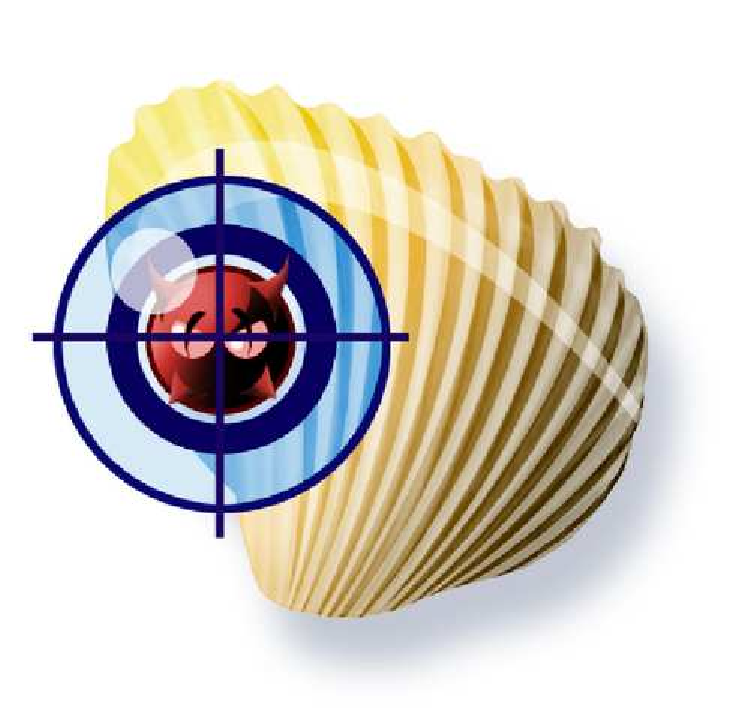
\includegraphics[width=353pt]{clam}
\vspace{3cm}
\begin{flushright}
  \rule[-1ex]{8cm}{3pt}\\
  \huge Signature configuration UI\\
        \huge \emph{User Manual}\\
\end{flushright}
\newpage
\setcounter{page}{1}
\pagestyle{fancy}
\tableofcontents
\vspace{1.0cm}
\noindent
\begin{boxedminipage}[b]{\textwidth}
    ClamAV for Windows - Signature configuration UI - User Manual,\\
    \copyright \  2010 Sourcefire, Inc.\\
    Authors: T\"{o}r\"{o}k Edvin\\
    This document is distributed under the terms of the GNU General
    Public License v2.\\

    Clam AntiVirus is free software; you can redistribute it and/or modify
    it under the terms of the GNU General Public License as published by
    the Free Software Foundation; version 2 of the License.\\

    This program is distributed in the hope that it will be useful,
    but WITHOUT ANY WARRANTY; without even the implied warranty of
    MERCHANTABILITY or FITNESS FOR A PARTICULAR PURPOSE.  See the
    GNU General Public License for more details.\\

    You should have received a copy of the GNU General Public License
    along with this program; if not, write to the Free Software
    Foundation, Inc., 51 Franklin Street, Fifth Floor, Boston,
    MA 02110-1301, USA.
\end{boxedminipage}

\vspace{0.3cm}
\noindent
\begin{boxedminipage}[b]{\textwidth}
    ClamAV and Clam AntiVirus are trademarks of Sourcefire, Inc.
\end{boxedminipage}
\setlength{\parindent}{18pt}
%\mainmatter

% !TeX root = sigui-manual.tex
\chapter{Overview}

\ClamAV allows users to deploy and use their own (or third party) virus signatures in
addition to the official virus signatures.
The virus signature database updater (\gls{freshclam}) can also be adapted to the
user's environment.

This is usually done by editing the configuration file \gls{freshclam.conf}, and copying the custom signatures to the database
directory.

However \CW protects the database directory against changes, even if those changes are attempted by a user with \emph{Administrator} privileges. 
A new tool is needed to make these changes: \textbf{Signature configuration UI} (SigUI).

\section{Features}
Using \emph{SigUI} an \emph{Administrator} can:
\begin{itemize}
\item Configure \gls{freshclam} to use a proxy
\item Configure which mirror \gls{freshclam} should use
\item Configure updates of custom signatures by \gls{freshclam}
\item Manually copy virus signature databases to \ClamAV's database directory
\item Deploy an existing \gls{freshclam.conf} \footnote{created using SigUI} to multiple machines
\end{itemize}

\section{Using SigUI}
\subsection{Launching the application}

The application can be launched from the \emph{Start Menu}:
Start $\to$ All Programs $\to$ ClamAV for Windows $\to$ SigUI 
\includegraphics{sigui_menu.jpg}

Or you can navigate to the installation directory of \CW
\footnote{\texttt{C:\textbackslash Program Files\textbackslash ClamAV for Windows} by default},
and from the \texttt{clamav} subfolder launch \texttt{sigui.exe}:\\

\includegraphics{sigui_icon.jpg}

In either case you must run this program with administrative privileges.
On \emph{Windows Vista} and later you will get the UAC popup to grant Administrator privileges to the application \footnote{If you are running as a user that has Administrator privileges, this is a simple "I Allow/Continue" style popup, otherwise it asks you for a login and password of a user with Administrator privileges}. On earlier versions you will need to login as \verb+Administrator+.

\subsection{How it works}

When changing \gls{freshclam} settings via the UI, it first verifies that the
settings are syntactically correct, and saves them in \gls{freshclam.conf}.

When installing custom signatures, \verb+SigUI+ verifies that \ClamAV can successfully load the databases, and install only those that are successfully loaded.

Once the databases are successfully installed, a reload is queued. ClamAV for Windows will reload the databases the next time the system is idle. SigUI will show a notification when the reload happens.
% !TeX root = sigui-manual.tex
\lstset{breaklines=true,basicstyle=\footnotesize\ttfamily}
\chapter{Usage examples}
\section{Configuring a proxy}
\Gls{freshclam} by default attemps to connect to the Internet directly. If you can only access the Internet by using a proxy, then you should configure the proxy using SigUI.

If you have already configured a system wide proxy setting, then easiest is to just press the \emph{Retrieve system proxy settings} button on the \emph{Updater configuration} tab.
This will retrieve the proxy settings from Internet Explorer, and display them in the \emph{Proxy settings} section. 
If the settings are correct, click \emph{Save settings}.

You can also manually input the proxy settings:
\label{sec:proxysettings}
\begin{itemize}
\item Tick the \emph{Proxy required for Internet access} checkbox
\item Set the proxy server and port in the \emph{Proxy server:} and \emph{Proxy port:} fields
\item If the proxy requires a username and password, then tick the \emph{Authentication required} checkbox
\begin{itemize}
\item Enter the username in the \emph{Proxy username:} field
\item Enter the password in the \emph{Proxy password:} field \footnote{Note that the password will be saved as cleartext in \gls{freshclam.conf}}
\end{itemize}
\item Check that the settings are correct
\item Click \emph{Save settings}
\end{itemize}

To test whether the proxy settings work, click \emph{Run freshclam to test configuration}.
This will run \gls{freshclam}, and display an error if it failed to connect through the proxy.
See \prettyref{sec:runfreshclam} for details.

\section{Choosing a mirror}
\label{sec:mirror}
\Gls{freshclam} by default uses the \gls{database.clamav.net} \gls{mirror}. Although this works well most of the time, you can get better download speeds by using a mirror from your country:
\begin{itemize}
\item Open SigUI
\item Open the \emph{Download Official Signatures from mirror} dropdown \footnote{
On the \emph{Updater configuration} tab, in the \emph{Signature sources} section}
\item Mirrors are of the form \texttt{db.XY.clamav.net}, where \emph{XY} is your two-letter country-code
\item Select the mirror corresponding to your country
\item Click \emph{Save settings}
\end{itemize}

You can also enter the \gls{hostname} of the mirror you wish to use, instead of choosing one from the dropdown. 
This mirror can be a server on your own network too. See \prettyref{sec:localmirror}.

\section{Deploying custom signature updates}
\label{sec:customsigs}
In addition to the official virus signatures, you can use your own signatures, or signatures provided by third-parties.
To deploy them you have these choices:
\begin{itemize}
 \item Put your custom signatures on your own webserver. See \prettyref{sec:customweb}
 \item Put your custom signatures on a network share. See \prettyref{sec:customnet}
 \item Manually copy your custom signatures each time you change them. See \prettyref{sec:custommanual}
 \item Write and deploy a script that copies the signatures to a local drive, and runs SigUI in command-line mode. See \prettyref{sec:customautomatedcopy}
\end{itemize}

A reload of the signatures is queued once the signatures are installed. See \prettyref{sec:updatenow}.

\subsection{Deploying your own signatures from a webserver}
\label{sec:customweb}
If you have written your own signatures and want to deploy them to multiple
\CW installations on your network, then the easiest is to put the signatures on your webserver (in your LAN).

The custom signature can be in any format that \gls{ClamAV} understands.
See \url{http://www.clamav.net/doc/latest/signatures.pdf} section 3 "Signature formats" for details about the format.
All the signature files, except CVD, are ASCII files. Both Unix (LF) and Windows-style (CR+LF) line-endings are accepted.
CVD files are binary files though, so you should not modify them.
The format of signatures is determined based on the database extension (in a case insensitive manner), so you must make sure to preserve the file's contents and
extension when copying it. (You can safely rename the file, as long as you preserve the extension).

Since these files are not digitally signed \footnote{Official \gls{CVD} files are digitally signed}, it is your responsibility to ensure that the signature files are not altered (by malware, etc.).

Deploying a new signature file is easy:
\begin{itemize}
\item Copy the signature to your webserver, at a location of your choice
\item Open SigUI
\item Click the \emph{Add} button next to the \emph{Custom signature URLs} section
\item Enter the full URL to your new signature file
\item Click OK.
\item Click \emph{Save settings}
\item See \prettyref{sec:ui_urladd} for details
\item You can repeat this operation on each machine that has \CW installed, or you can automate it, see \prettyref{sec:deploy_conf}
\end{itemize}

\subsection{Deploying your own signatures from a network share}
\label{sec:customnet}
This is similar to downloading a signature file from a webserver, see \prettyref{sec:customweb}.
Except you have to add an \gls{UNC path} instead of an \verb+http://+ URL.

However \CW requires this \gls{UNC path} to be readable by the \gls{SYSTEM account}.
Usually network shares, and network mapped drives are not accessible to this user.
If you have made them accessible (it is out of scope for this document to discuss how), then you can of course use them in SigUI.

\subsection{Deploying third-party signatures}

If you want to deploy third-party signatures that are not in \gls{CVD} format \footnote{freshclam supports third-party signatures in CVD format, but there are no such signatures yet}, you can do so with some additional steps:
\begin{itemize}
\item Download the third-party signatures to your server
\item Check their integrity by comparing against the third-party supplied checksum and digital signatures. There usually are scripts to accomplish this
\item Copy the signatures to your webserver, at a location of your choice
\item Make sure you preserve the extension of the files, as the signature format is determined based on the extension
\item Add the full URL path to these signatures to \gls{freshclam.conf} using \gls{SigUI}.
See \prettyref{sec:ui_urladd}
\end{itemize}

Note that if you add third-party signatures memory usage will increase (depending on the complexity and size of the signatures), and performance may be different.

Note that the downloaded signature files will all be placed in the same directory. Hence you must make sure you don't have two URLs that, when downloaded, have the same filename.
The UI will warn you if you try to do that\footnote{the two URLs with same filenames will just keep overwriting the same file}.

\subsection{Manually copying custom signatures to database directory}
\label{sec:custommanual}
If you want \gls{ClamAV} to use a custom signature, you just need to copy it to its database directory. However, as explained earlier in this document, that directory is protected against changes so you need to use SigUI to copy the databases.

This can be achieved by using the \emph{Local signature management} tab:
\begin{itemize}
\item Click \emph{Add}
\item This will open the standard \emph{Open file(s)} dialog
\item Select the file(s) you want to add
\item Click \emph{Open}
\item The files will show up in the \emph{New signatures} list
\end{itemize}

At this point the files haven't been installed yet.
The databases currently installed can be seen in the \emph{Installed signatures} list.
By default you should see \verb+main.cvd+,\verb+daily.cvd+, and \verb+bytecode.cvd+
\footnote{Or .cld once they are updated. CVD files change into CLD files upon an update.
Of course if the updater didn't run yet you won't see any files there}.

You want your new signatures to show up in the \emph{Installed signatures}, so the next step is clicking on \emph{Verify and Install signatures}.
This will perform the following:
\begin{itemize}
\item Copy all the signatures to a (protected) temporary staging directory \footnote{\texttt{clamav\textbackslash staging\_dir} subdirectory}.
\item Test the signatures by loading each one\footnote{Using \texttt{libclamav.dll} only, they are not loaded in the realtime engine}. CVD files also have their digital signature checked.
\item The signatures that pass verification are installed in the real database directory
\item \CW will load them the next time it updates the database (usually once ah hour)
\item If there are signatures that fail verification an error message will be shown, with details on why the signatures failed to load.
\end{itemize}

\subsection{Removing signature files}
\label{sec:localremove}
If you want to remove one of your signatures, you can select the file in the \emph{Installed signatures} list, and click \emph{Delete}. This will erase the file from the disk!
Note that you can delete the files automatically downloaded by \gls{freshclam} too, but they will just reappear at the next update.  The only file you can't delete is \gls{daily.cvd} and \gls{daily.cld}.
The presence of one these files is essential to the proper operation of the \gls{ClamAV} engine.

\subsection{Automating signature and configuration file deployments on a network}
\label{sec:customautomatedcopy}
\label{sec:deploy_conf}

The graphical mode of SigUI is useful for making local changes to \gls{freshclam.conf} and the database directory. However if you want to automate the process (call it from a script), there is a commandline interface too:
\begin{itemize}
	\item You must run it as Administrator user. Otherwise you get the \gls{UAC} popup, which is not what you want in a script.
	\item If you want to copy signatures to the database directory:
		\begin{itemize}
			\item Create a file \verb+signatureslist+ with the full path to the signatures you want to install, one on a line. Don't quote or escape the filenames, just write them as is.
			\item Run:
\begin{lstlisting}
"C:\Program Files\ClamAV for Windows\clamav\SigUI.exe" -i <signatureslist
\end{lstlisting}
			\item Another alternative is to pipe it the output of another program \footnote{Interactively entering the filenames from the commandprompt won't work}:
\begin{lstlisting}
echo '<databasepath>' | "C:\Program Files\ClamAV for Windows\clamav\SigUI.exe" -i
\end{lstlisting}
			\item SigUI will test each database by loading them, and prints progress messages to the standard output.
			\item SigUI will print error messages on failed database loads to the standard error
			\item The exitcode will be 0 if all signatures were successfully installed, and nonzero if some signatures failed to install
		\end{itemize}
Note that using \gls{freshclam}'s support for custom signature URLs is usually a better solution, you will only need to deploy the modified \gls{freshclam.conf}.
\item Deploying a modified \gls{freshclam.conf}:

\begin{itemize}
\item Create a \gls{freshclam.conf} on one machine with \gls{SigUI}
\item Test it, see \prettyref{sec:runfreshclam}
\item Write a script to automatically invoke \verb+SigUI.exe+ on each machine on your network (for example using a logon script, or a \verb+msi+ installer)
\item Have it execute this command:
\begin{lstlisting}
"C:\Program Files\ClamAV for Windows\clamav\SigUI.exe" -w <new\_freshclam.conf
\end{lstlisting}
\item Alternatively you can pipe it the freshclam.conf:
\begin{lstlisting}
somecommand | "C:\Program Files\ClamAV for Windows\clamav\SigUI.exe" -w
\end{lstlisting}

\item SigUI will test the config file for syntactic correctness, and install it if it is valid
\end{itemize}
\end{itemize}

\section{Setting up a local mirror}
\label{sec:localmirror}

If you have a lot of ClamAV installations on your local network, then you can setup \gls{freshclam} as described in the answer for  \emph{I’m running ClamAV on a lot of clients on my local network} at \url{http://www.clamav.net/lang/en/support/faq/faq-cvd/}.
Once you've setup the local mirror you can configure it:
\begin{itemize}
\item Open SigUI
\item Enter the hostname, or IP address of your local mirror in the \emph{Download official signatures from mirror:} field
\item Click \emph{Save settings}
\item Click \emph{Run freshclam to test configuration}. See \prettyref{sec:runfreshclam}
\end{itemize}

Another option is to setup a caching proxy, and set ClamAV to use that. See \prettyref{sec:proxysettings}.

% !TeX root = sigui-manual.tex
\chapter{User interface}
\section{Run freshclam to test configuration}
\label{sec:runfreshclam}
\section{Custom URLs}
\label{sec:ui_urladd}
The \emph{Custom signature URLs} section on the \emph{Updater configuration}
page allows you to add custom URLs.

Freshclam will automatically download these each time it updates the official signatures (usually once an hour).
If you webserver supports \verb+If-Modified-Since+ headers, it will only
download the new database if it is newer than the already installed one.

Digital signatures  are checked only for \gls{CVD} signatures\footnote{because they are the only ones that contain such signatures}.
Freshclam automatically tests all signatures (for syntactic correctness) after downloading, but
before installing them. If a signature file is malformed it is not installed and
an error is logged.

Usage:
\begin{itemize}
\item Click Add to add a new URL, press OK when done
\item If the URL is not in the correct format, an error message is shown.
Correct the URL and press OK again.
\item The new URL shows up in the \emph{Custom signature URLs} section
\item Add as many URLs as needed
\item You can remove an URL by clicking the \emph{Remove} button.
\textbf{WARNING}: If the database was already downloaded it won't remove the downloaded signature file from the disk.
See \prettyref{sec:localremove} on how to do that.
\item Check that you entered the correct URLs.
\item Click \emph{Save settings}.
\item Click \emph{Run freshclam to test configuration} to make sure freshclam is
able to correctly download the signatures. Freshclam will only install
signatures that are in the syntactically correct.
See \prettyref{sec:runfreshclam}
\end{itemize}

Note that the downloaded signature files will all be placed in the same directory. Hence you must make sure you don't have two URLs that, when downloaded, have the same filename.
The UI will warn you if you try to do that. \footnote{the two URLs with same filenames will just keep overwriting the same file}.
\section{Update now}
\label{sec:updatenow}

\section{Removing signature files}
\label{sec:localremove}

% !TeX root = sigui-manual.tex
\chapter{Copyright and License}
The Signature configuration UI is released under the GNU General Public License
version 2.

{\footnotesize
\begin{verbatim}
Copyright (C) 2010 Sourcefire, Inc.

This program is free software; you can redistribute it and/or modify
it under the terms of the GNU General Public License version 2 as
published by the Free Software Foundation.

This program is distributed in the hope that it will be useful,
but WITHOUT ANY WARRANTY; without even the implied warranty of
MERCHANTABILITY or FITNESS FOR A PARTICULAR PURPOSE.  See the
GNU General Public License for more details.

You should have received a copy of the GNU General Public License
along with this program; if not, write to the Free Software
Foundation, Inc., 51 Franklin Street, Fifth Floor, Boston,
MA 02110-1301, USA.
\end{verbatim}
}


%\backmatter

% INDEX - disabled for now, since it is not needed
%\cleardoublepage
%\phantomsection %needed so that Index shows up in TOC
%\addcontentsline{toc}{chapter}{Index}
%\printindex
\end{document}
